
\section{\textcolor{black}{Uncertainty sources}} % Sections are added in order to organize your presentation into discrete blocks, all sections and subsections are automatically output to the table of contents as an overview of the talk but NOT output in the presentation as separate slides

%------------------------------------------------


\begin{frame}
	\frametitle{Real world with uncertainties}
\begin{columns}
    \column{0.5\textwidth}    \animategraphics[autoplay,loop,width=7.2cm]{3}{figures-gif/typhoon/Typhoon-}{1}{39}    \footnotetext{\href{https://en.wikipedia.org/wiki/Weather_Research_and_Forecasting_Model}{Source: Wikipedia}}
    \column{0.5\textwidth} 
    \begin{figure}
    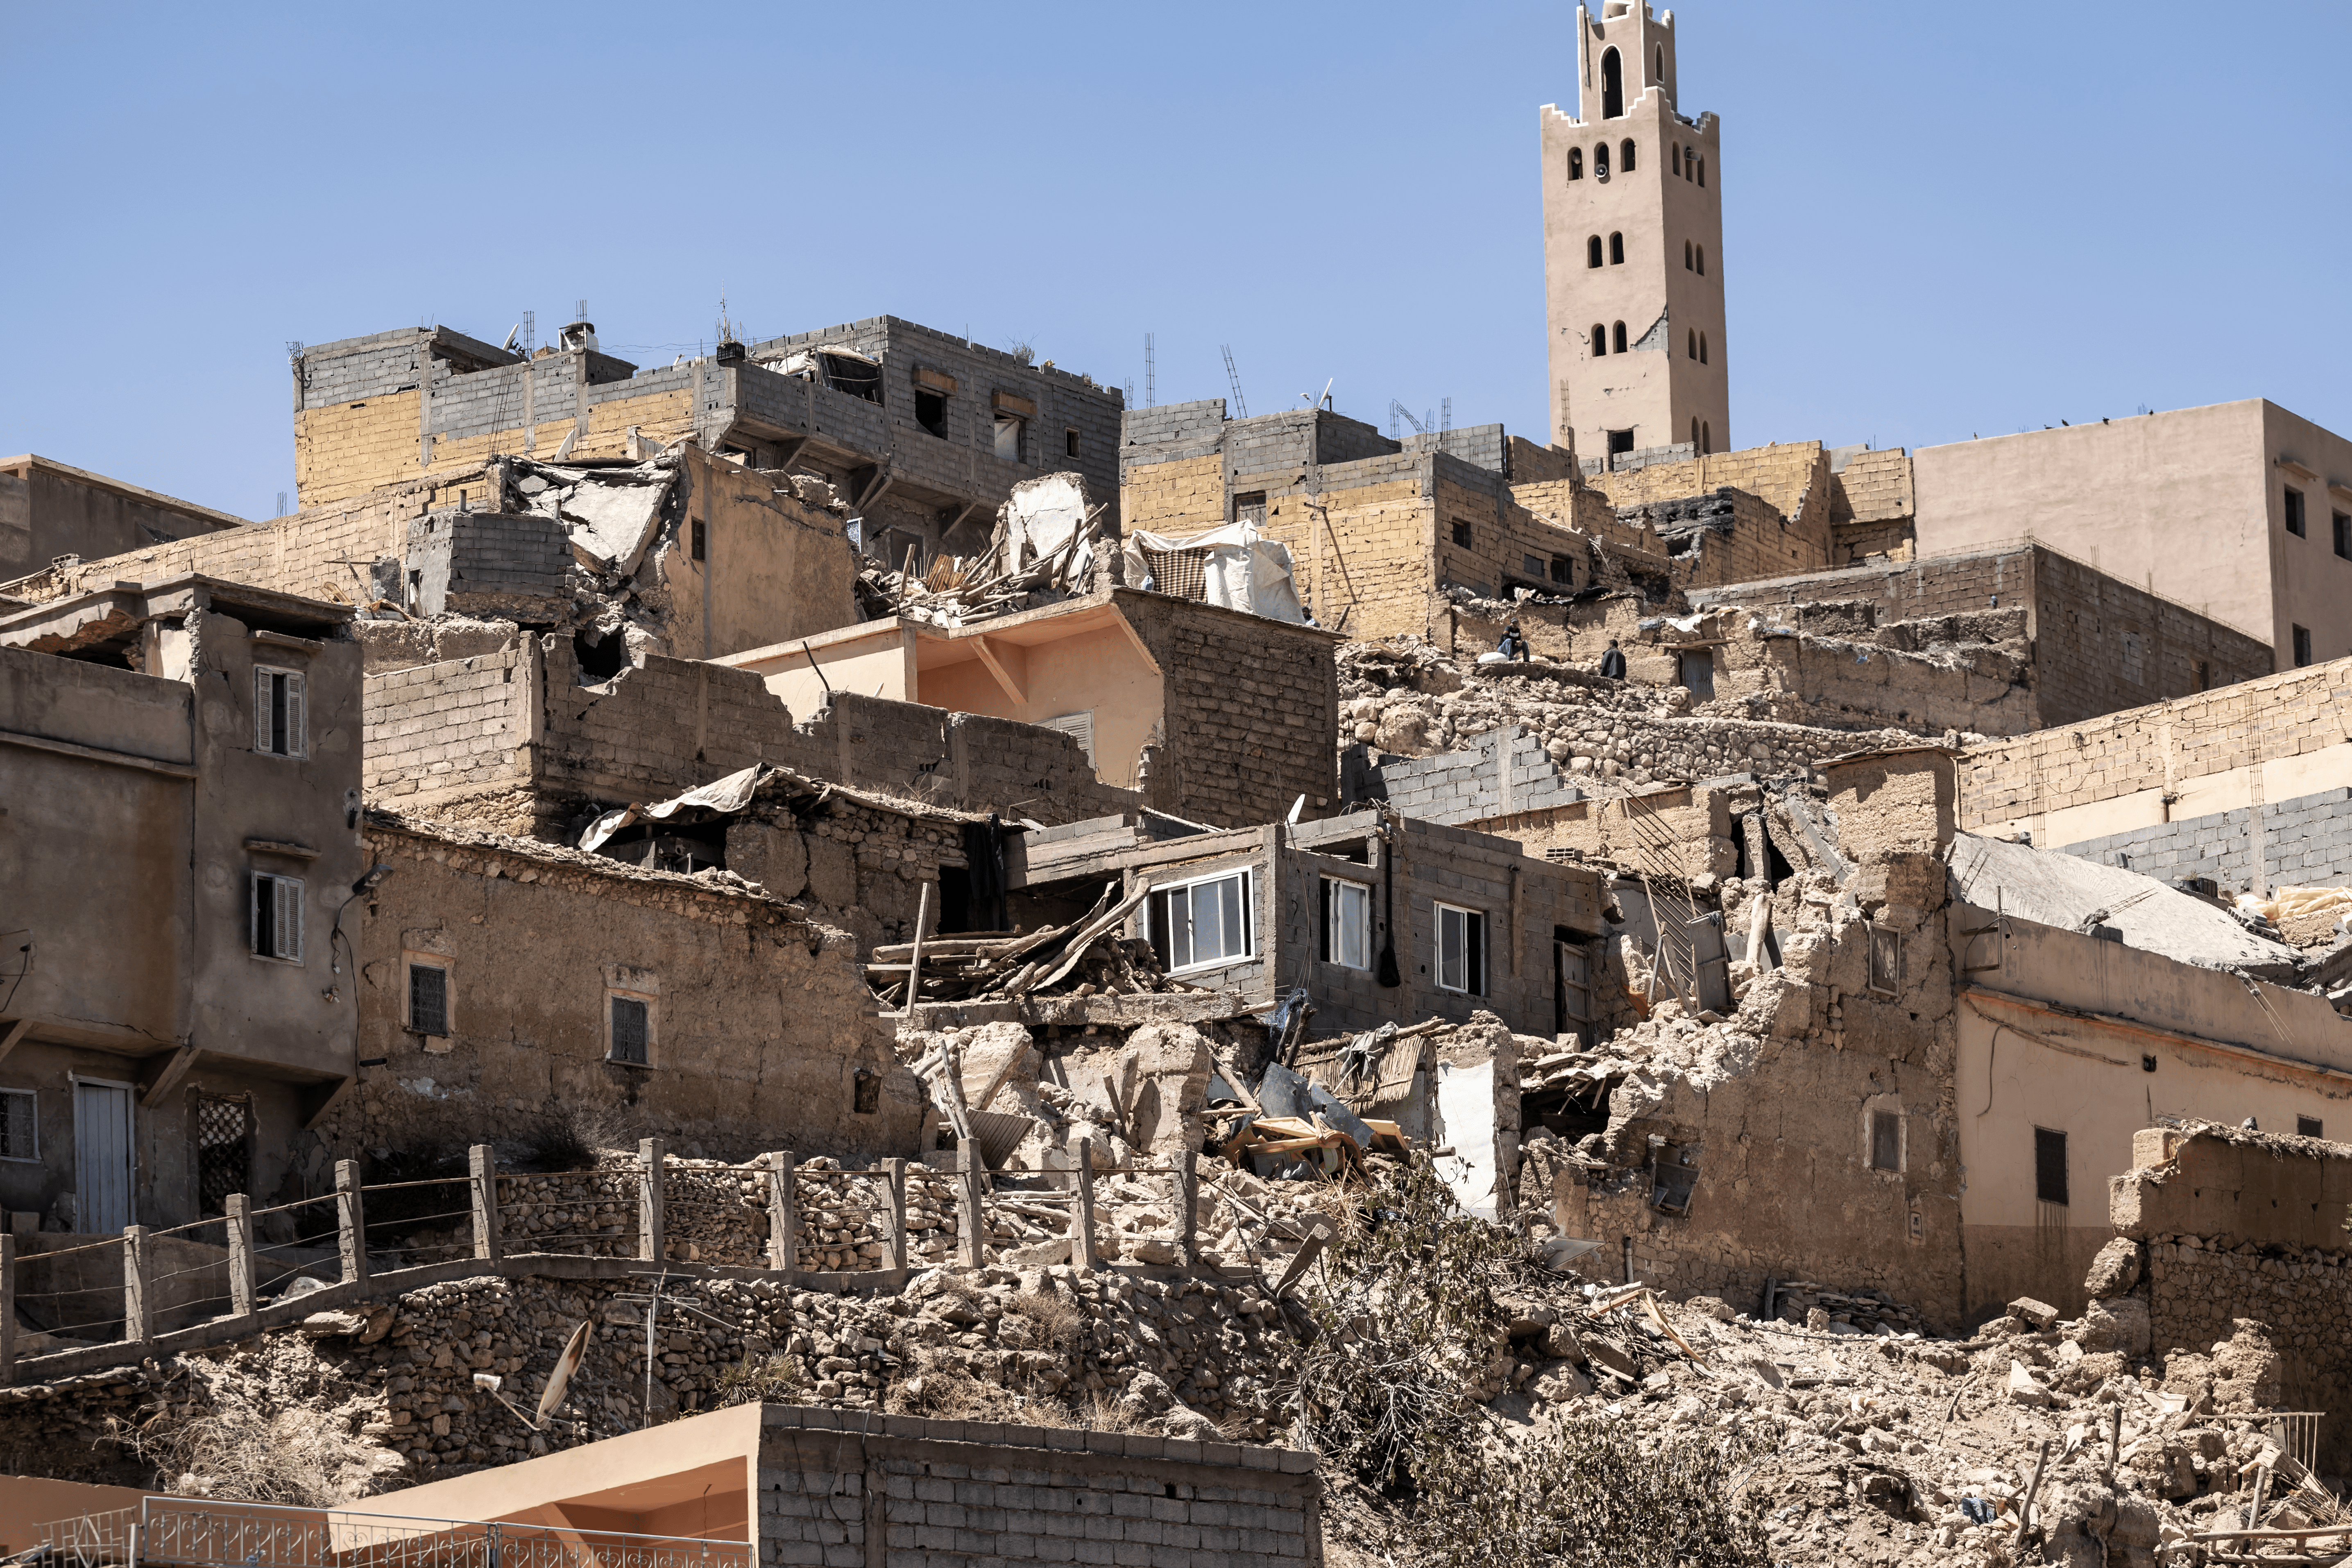
\includegraphics[width = 5.3cm]{figures/figure-earthquake.png}    
    \includegraphics[width = 5.3cm]{figures/figure-embankment.png}    
    \end{figure}    
\end{columns}
\end{frame}

%------------------------------------------------
\begin{frame}
\frametitle{Types of two uncertainties}
\framesubtitle{Aleatoric vs epistemic}

\begin{columns}
    \column{0.7\textwidth}
        \begin{figure}
        \centering
            \includegraphics[width = 9cm]{figures/aleatoricvsepisidemic.pdf}
            \caption{Aleatoric uncertainty vs Epistemic uncertainty}
        \end{figure} 
    \column{0.3\textwidth}
     \textbf{Distinguish}:
     \begin{block}{Aleatoric uncertainty}
statistical variability, inherently random effects (\textbf{irreducible})
     \end{block}
     \begin{block}{Epistemic uncertainty}
model uncertainty, a lack of knowledge (\textbf{reducible})
     \end{block}    
    \end{columns}
\end{frame}


%--------------------------------------------------

\begin{frame}
\frametitle{Type one: aleatoric uncertainty}
 \centering
  \begin{figure}
    \includegraphics[scale=0.65]{figures/figure-coin_shooting.pdf}
\end{figure}
\end{frame}

%----------------------------------------------------------


\begin{frame}
\frametitle{Type two: epistemic uncertainty}
    \begin{columns}[]       
        
    \column{0.5\textwidth}  
        \centering

        \begin{figure}
            \includegraphics[scale=0.8]{figures/figure-table_ruler.pdf}
        \end{figure}
 
      

    \column{0.5\textwidth}
    \only<1>{    
     
    \textbf{Random variables: }

    $x_{i} = x^{\star} (\text{10m}) \pm \epsilon$, $\epsilon \sim \mathcal{N}(0,\sigma^2)$

    $ x_{i} \sim iid$

    $\boldsymbol{x} = (x_1,x_2,\cdots,x_n)$
    \bigskip
    
   \textbf{First moment:} 

   \begin{equation}
   \begin{aligned}
      \mathbb{E}(\boldsymbol{x}) &= \frac{1}{n} \sum_{i=1}^{n} x_i \\
       &= \mathbb{E}(x^{\star}) (\text{10m}) +\mathbb{E}(\boldsymbol{\epsilon})\\  
   \end{aligned}
   \end{equation} 
   \pause
When $n \rightarrow \infty$, $\mathbb{E}(\boldsymbol{x}) \approx x^{\star} + 0 \approx$ 10 (m)
    
    }

         \only<2>{
        \begin{figure}
            \includegraphics[scale=0.8]{figures/table-ruler_PDF.pdf}
            \caption{PDF with increasing trails}
        \end{figure}
        } 


 
\end{columns}
\end{frame}

%----------------------------------------------------------


\begin{frame}
\frametitle{Uncertainty components:}
\Large\textbf{Total uncertainty $\approx$ aleatoric uncertainty $+$ epistemic uncertainty}

\begin{columns}

\column{0.6\textwidth}
\begin{figure}
\includegraphics[scale=2.5]{figures/figure-total_Uncertainty.pdf}
\end{figure}
\column{0.4\textwidth} 
Not simple as it shows:
\centering
\begin{figure}
\includegraphics[scale=0.5]{figures/figure-uncertainty_classification.png}
\end{figure}
\footnotetext{Source:$\hyperlink{https://www.linkedin.com/pulse/aleatory-epistemic-uncertainty-software-development-projects-alleman/}{link}$} 
\end{columns}   
\end{frame}

%----------------------------------------------------------
\begin{frame}
\frametitle{What uncertainties we have in geotechnical engineering exactly?}
\framesubtitle{Mix of aleatoric and epistemic}
    \begin{figure}
    \includegraphics[scale=1]{figures/figure-UQtype1.pdf}    
    \hfill
    \includegraphics[scale=0.4]{figures/figure-UQtype2.pdf}
    \footfullcite{zdravkovic2020}
    \hfill
    \includegraphics[scale=0.6]{figures/figure-UQtype3.pdf}
    \footfullcite{nagel2020}
    \hfill
    \includegraphics[scale=0.9]{figures/figure-UQtype4.pdf}    
    \end{figure}

\end{frame}